The Orlin's strongly polynomial algorithm \cite{orlin1993faster} is a modification of the capacity scaling  approach. Here we need the similiar assumptions as in the previous algorithms.


\begin{assumption}\label{ass:cost_nonnegativity_orlin}
    All arc costs are nonnegative.
\end{assumption}


\begin{assumption}\label{ass:one_scc_orlin}

For each pair of nodes $i, j \in V$, there is a directed path from $i$ to $j$ in graph $G$.
\end{assumption}

These two assumptions are the same as \Cref{ass:one_scc} and \Cref{ass:cost_nonnegativity}. Here we need one additional assumption. We need to assert that the network is uncapacitated.

\begin{assumption}\label{ass:uncapacitated_orlin}
    A given network is \textbf{uncapacitated} that is, the instance of a problem consists only of graph $G$ and arc costs $c$.
\end{assumption}

In \Cref{sec:uncapacitated} we present a reduction from a capacitated instance to an uncapacitated one. Since we modify the network by adding a node for each edge, the time complexity may be worse. In order to prevent this, we need to use a modified shortest path algorithm described in \Cref{sec:modified_spp}.

\Cref{alg:capacity_scaling} follows the capacity scaling approach for capacitated networks. Due to the modification, we get some useful properties.

\begin{lemma}[Lemma 5 in \cite{orlin1993faster}]
At every step of an uncapacitated version of the algorithm, the flow and the residual capacity of every arc in the residual network is an integral multiple of the scale factor $\Delta$.
\end{lemma}
This property allows us to eliminate the augmentations performed at line~$7$ of \Cref{alg:capacity_scaling}.

\section{Idea}

Unlike the standard capacity scaling approach, this algorithm solves \textbf{the dual minimum cost flow problem}, as described in \Cref{dualdef}. It first computes the optimal node potentials and subsequently uses them to derive an optimal flow. 

Several modifications to the traditional capacity scaling algorithm are required to achieve the desired result.

First, we introduce the concept of \textit{contraction}. The intuition behind this is that if the flow $x_{ij}$ across an arc $(i,j)$ is sufficiently large, $x_{ij}$ will remain positive until a feasible flow is found. Consequently, by complementary slackness (\Cref{comp_slack}), the reduced cost will always satisfy $c_{ij}^\pi = 0$. This allows us to merge nodes $i$ and $j$.

Next, we present a scenario where the capacity scaling algorithm with contraction fails to be strongly polynomial, and we introduce Orlin's approach to overcome this limitation.

Following this, the augmentation loop remains largely identical to that of the standard capacity scaling algorithm. However, if the capacitated minimum cost flow problem is reduced to an uncapacitated one, the shortest path computation can be optimized to improve the overall time complexity.

Finally, we must \textit{uncontract} the nodes and compute the actual flow. Because the algorithm initially solves the dual problem, it yields only the optimal potentials $\pi^*$. Using these potentials, we construct an auxiliary network $G'$ containing only the arcs $(i,j)$ from $G$ whose reduced costs $c_{ij}^{\pi^*}$ are exactly $0$. According to \Cref{comp_slack}, only these arcs can carry positive flow. Therefore, determining the optimal flow simply requires executing a maximum flow algorithm on $G'$.

We elaborate on these steps in detail below.

\subsection{Contraction}\label{sec:contraction}
In this section, we detail the contraction operation, which was originally introduced by Orlin \cite{orlin1993faster}. Recall that we contract only those arcs guaranteed to carry positive flow in all subsequent phases. By \Cref{comp_slack}, this contraction does not affect optimality.

The contraction operation proceeds as follows. Assuming we can compare node identifiers, let $i < j$ without loss of generality. For every arc $(i,j)$ meeting the condition for positive flow, we \textit{contract} node $j$ into node $i$ by performing the following substitutions:
\begin{itemize}
    \item set $b(i) \gets b(i) + b(j)$ and $e(i) \gets e(i) + e(j)$,
    \item replace every arc $(v,j)$ with the arc $(v,i)$,
    \item replace every arc $(j,v)$ with the arc $(i,v)$,
    \item assign the new arcs the same costs as the arcs they replace,
    \item remove node $j$.
\end{itemize}

We must also determine a threshold flow value that guarantees the flow along an arc will remain positive until a feasible flow is found.

During a $\Delta$-scaling phase, at most $n$ augmentations can occur. Suppose an arc $(i,j)$ is the residual arc augmented each time; its flow would change by at most $n\Delta$ units. Summing over all subsequent phases, the total flow change for any arc is bounded by $n(\Delta + \Delta/2 + \Delta/4 + \dots + 1) < 2n\Delta$. Consequently, any arc $(i,j) \in E$ whose flow exceeds $2n\Delta$ during a $\Delta$-scaling phase is guaranteed to maintain a positive flow in all subsequent phases. We define such arcs as \textit{strongly feasible}.

\begin{defn}[Strongly feasible arc \cite{orlin1993faster}]\label{def:strongly_feasible}
    Let $x_{ij}$ denote the flow across the arc $(i,j)\in E$ during a $\Delta$-scaling phase. The arc $(i,j)$ is called \textbf{strongly feasible} if $x_{ij} \geq 2n\Delta$.
\end{defn}

Because the contraction process itself may induce an additional augmentation, we establish the following lemma to adjust our bound.

\begin{lemma}[Lemma 11 in \cite{orlin1993faster}]
In a $\Delta$-scaling phase, if $x_{ij} \geq 3n\Delta$ for some arc $(i,j)$ in $\hat{E}$, then $x_{ij} > 0$ in all subsequent scaling phases.
\end{lemma}

\begin{proof}[Proof (from {\cite[p.~346]{orlin1993faster}})]
    Without contractions, the flow change on any arc due to augmentations across all subsequent scaling phases is at most $n(\Delta + \Delta/2 +\Delta/4+ \dots + 1)$. Each contraction causes at most one additional augmentation, and there are at most $n-1$ contractions. Thus, the total flow change on any arc is strictly less than $3n\Delta$.
\end{proof}

Next, we describe the \textit{uncontraction} operation. Because computing the optimal flow requires the original network alongside the final node potentials, we must keep a record of every contraction. Furthermore, we must track how the potentials change across subsequent contractions to accurately compute the final potentials. Once the final potentials are obtained, we can calculate the reduced costs for each arc and proceed with the maximum flow algorithm, utilizing only the arcs that have a reduced cost of zero.


\subsection{A difficult case for the algorithm with contraction}\label{sec:pessimistic_orlin}

There is a specific scenario in which the time complexity of the algorithm might depend on $\log C$, where $C = \max \{ |b(i)| \colon i \in V \}$. Consider the following pathological example provided by Orlin \cite{orlin1993faster}:

\begin{figure}[H]
    \centering
    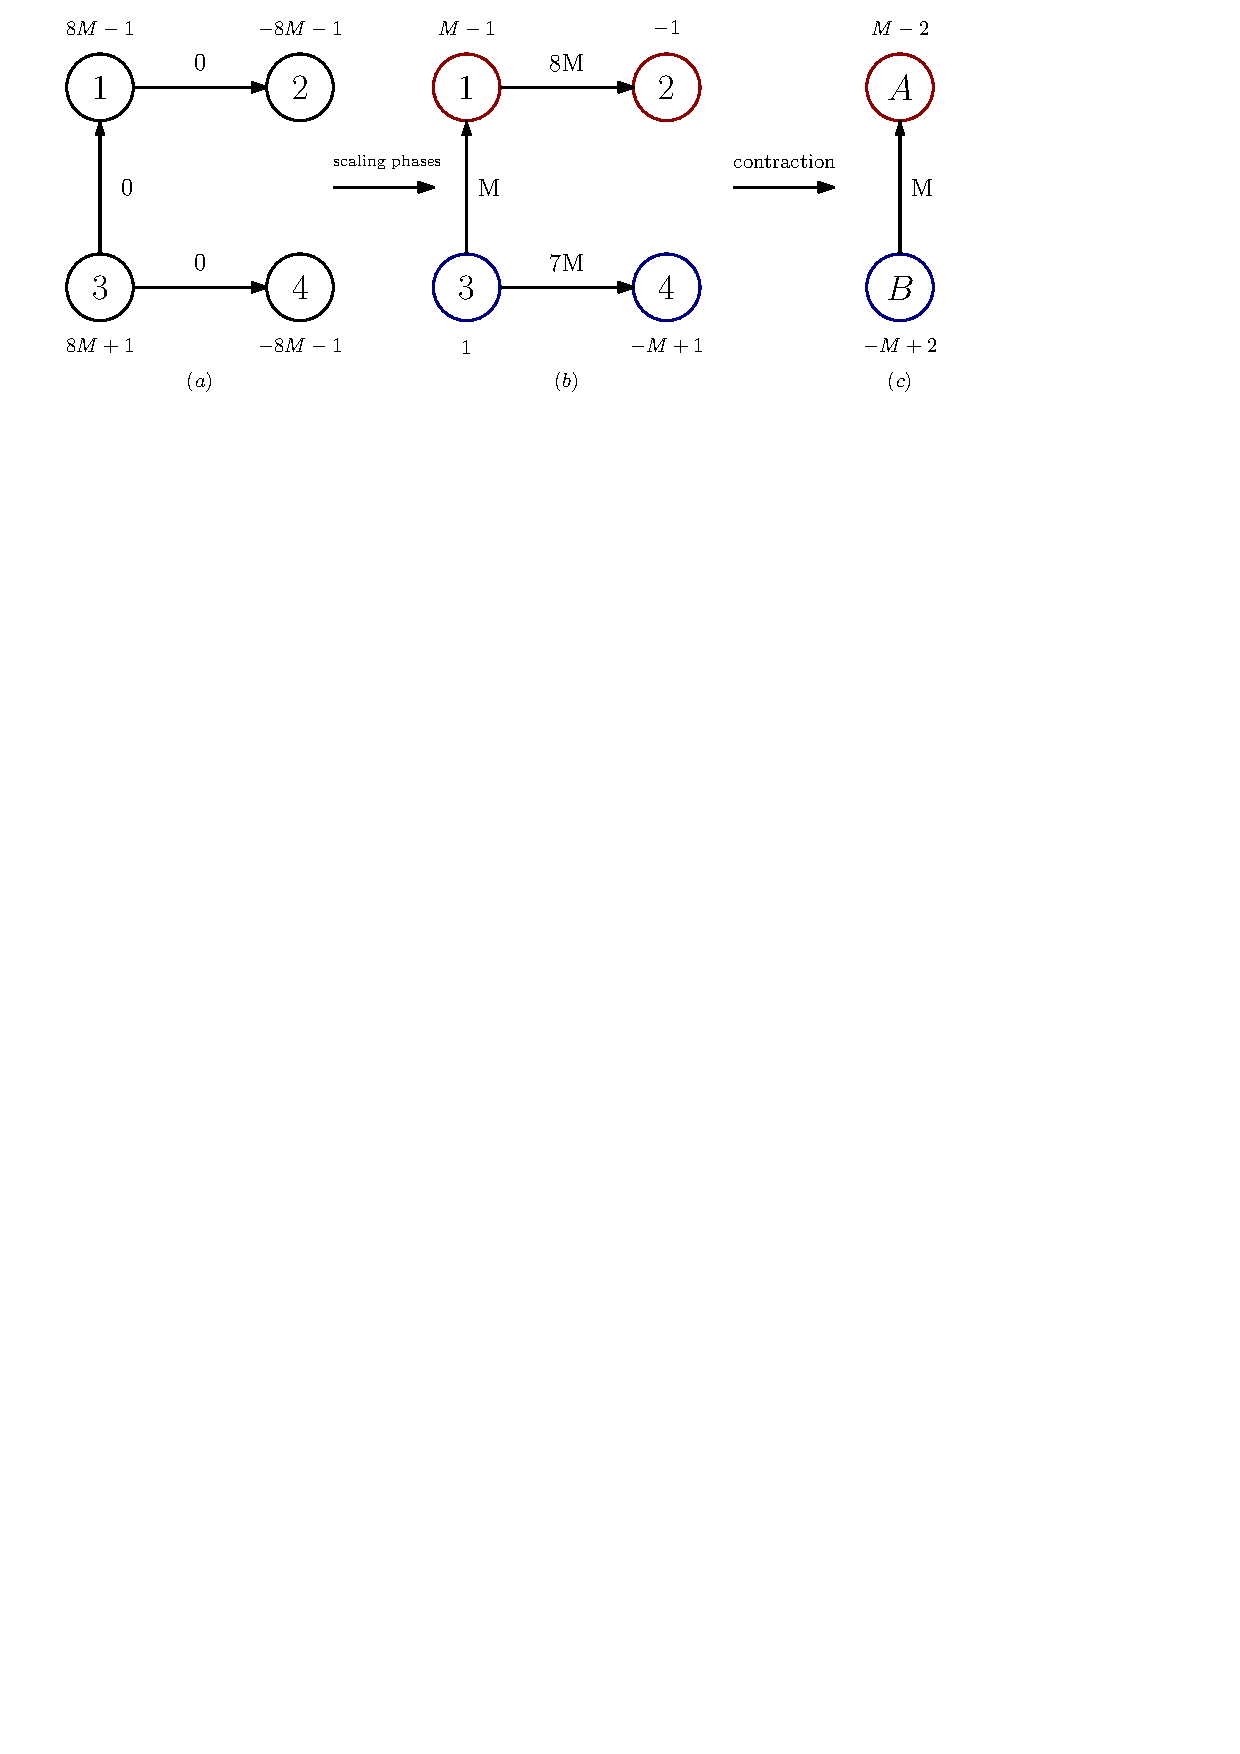
\includegraphics[width=0.8\linewidth]{chapters/orlin/img/pato-capacity.pdf}
    \caption{A hard case for the capacity scaling algorithm with contraction. Figure adapted from \cite{orlin1993faster}.}
    \label{fig:pathological}
\end{figure}

Let $M$ denote a sufficiently large number, specifically one that is exponentially larger than $n$ and $m$. In \Cref{fig:pathological}a, we present the initial supplies and demands. The algorithm with contractions performs the following sequence of augmentations:
\begin{itemize}
    \item ($8M$-scaling): \textsc{Augment}$(8M, 3 \rightarrow 2)$,
    \item ($4M$-scaling): \textsc{Augment}$(4M, 1 \rightarrow 4)$, 
    \item ($2M$-scaling): \textsc{Augment}$(2M, 1 \rightarrow 4)$,
    \item ($M$-scaling): \textsc{Augment}$(M, 1 \rightarrow 4)$.
\end{itemize}

The resulting state is illustrated in \Cref{fig:pathological}b. At this point, we can contract the arc $(1,2)$, as shown in \Cref{fig:pathological}c. However, achieving a feasible flow now requires $O(\log M)$ scaling phases. Consequently, the running time is no longer strongly polynomial.

This issue arises because it is possible to construct contracted nodes whose excess is close to $\Delta$, even though their original supply or demand remains significantly smaller. Orlin observes that these problematic cases occur when the excess satisfies $e(k) = \Delta - \epsilon$ and $b(k) = -\epsilon$, or symmetrically, when $e(k) = -\Delta + \epsilon$ and $b(k) = \epsilon$, for some arbitrarily small $\epsilon > 0$ \cite{orlin1993faster}. As a result, erasing the excess for such a node without further contractions requires a large number of augmentations to reach a feasible flow.

To overcome this difficulty, Orlin modifies the criteria for selecting active nodes for the sets $S(\Delta)$ and $T(\Delta)$. Specifically, a node $u$ is included only if its excess satisfies $|e(u)| \geq \alpha \Delta$, for some constant $\frac{1}{2} < \alpha < 1$ \cite{orlin1993faster}. Under this condition, we still augment $\Delta$ units of flow, but the total number of $\Delta$-scaling phases becomes independent of the magnitude of the excesses. 

Thus, in the strongly polynomial variant of the algorithm, we formally define the sets of active sources and sinks as $S(\Delta) = \{i \in V \colon e(i) \geq \alpha\Delta\}$ and $T(\Delta) = \{i \in V \colon e(i) \leq -\alpha\Delta\}$, respectively.

\subsection{Optimized shortest path algorithm}
\label{sec:modified_spp}

As in the previous algorithm, we utilize Fredman and Tarjan's implementation of Dijkstra's algorithm \cite{fredman1987} to compute the shortest paths. This implementation achieves a time complexity of $O(m + n\log n)$.

If the original network is capacitated, it must first be converted into an uncapacitated instance. We accomplish this using the reduction described in \Cref{sec:uncapacitated}. However, this reduction introduces $m$ additional nodes to the network, which inadvertently degrades the overall time complexity of the shortest path algorithm.

To overcome this issue, we can conceptually bypass these newly added vertices. For instance, we can identify them using a boolean flag. Observe that each added node $k$ is adjacent to exactly two original nodes, say $i$ and $j$. Note that, without loss of generality, if there is a residual arc from $k$ to $j$, with residual capacity $r_{kj} \geq \Delta$, then, instead of considering residual arcs $(i,k)$ and $(k,j)$, we can add one arc $(i,j)$ to the shortest path graph. This operation is visualized in \Cref{fig:optimized_shortest_path}. Thus we can effectively skip the intermediate node $k$ during the main computation. By doing so, we maintain a graph with only $O(n)$ vertices for the shortest path algorithm. Once the shortest path distances for all original vertices have been determined, the distance for any added vertex $k$ can be computed in $O(1)$ time using the relation $d(k) = \min \{ d(i) + c_{ik}, d(j) + c_{jk} \}$.

\begin{figure}[H]
    \centering
    \begin{tikzpicture}[
    >=Stealth,
    vertex/.style={circle, draw, minimum size=8mm, inner sep=0pt, font=\small},
    % elabel style ensuring horizontal text
    elabel/.style={fill=white, inner sep=1.5pt, font=\scriptsize, midway} 
]

\node[vertex] (i) at (0, 1) {$i$};
\node[vertex] (j) at (0, -1) {$j$};
\node[vertex] (k) at (3, 0) {$k$};

\draw[->] (i) -- (k);
\draw[->] (j) -- node[elabel] {$x_{jk} \ge \Delta$} (k);

\draw[->, thick, line width=1.5pt] (4.5, 0) -- (6.5, 0);

\node[vertex] (i_prime) at (8, 1) {$i$};
\node[vertex] (j_prime) at (8, -1) {$j$};

\draw[->] (i_prime) -- (j_prime);

\end{tikzpicture}
    \caption{Graph nodes shortest path optimization.}
    \label{fig:optimized_shortest_path}
\end{figure}

